% Created by tikzDevice version 0.7.0 on 2014-06-29 19:22:43
% !TEX encoding = UTF-8 Unicode
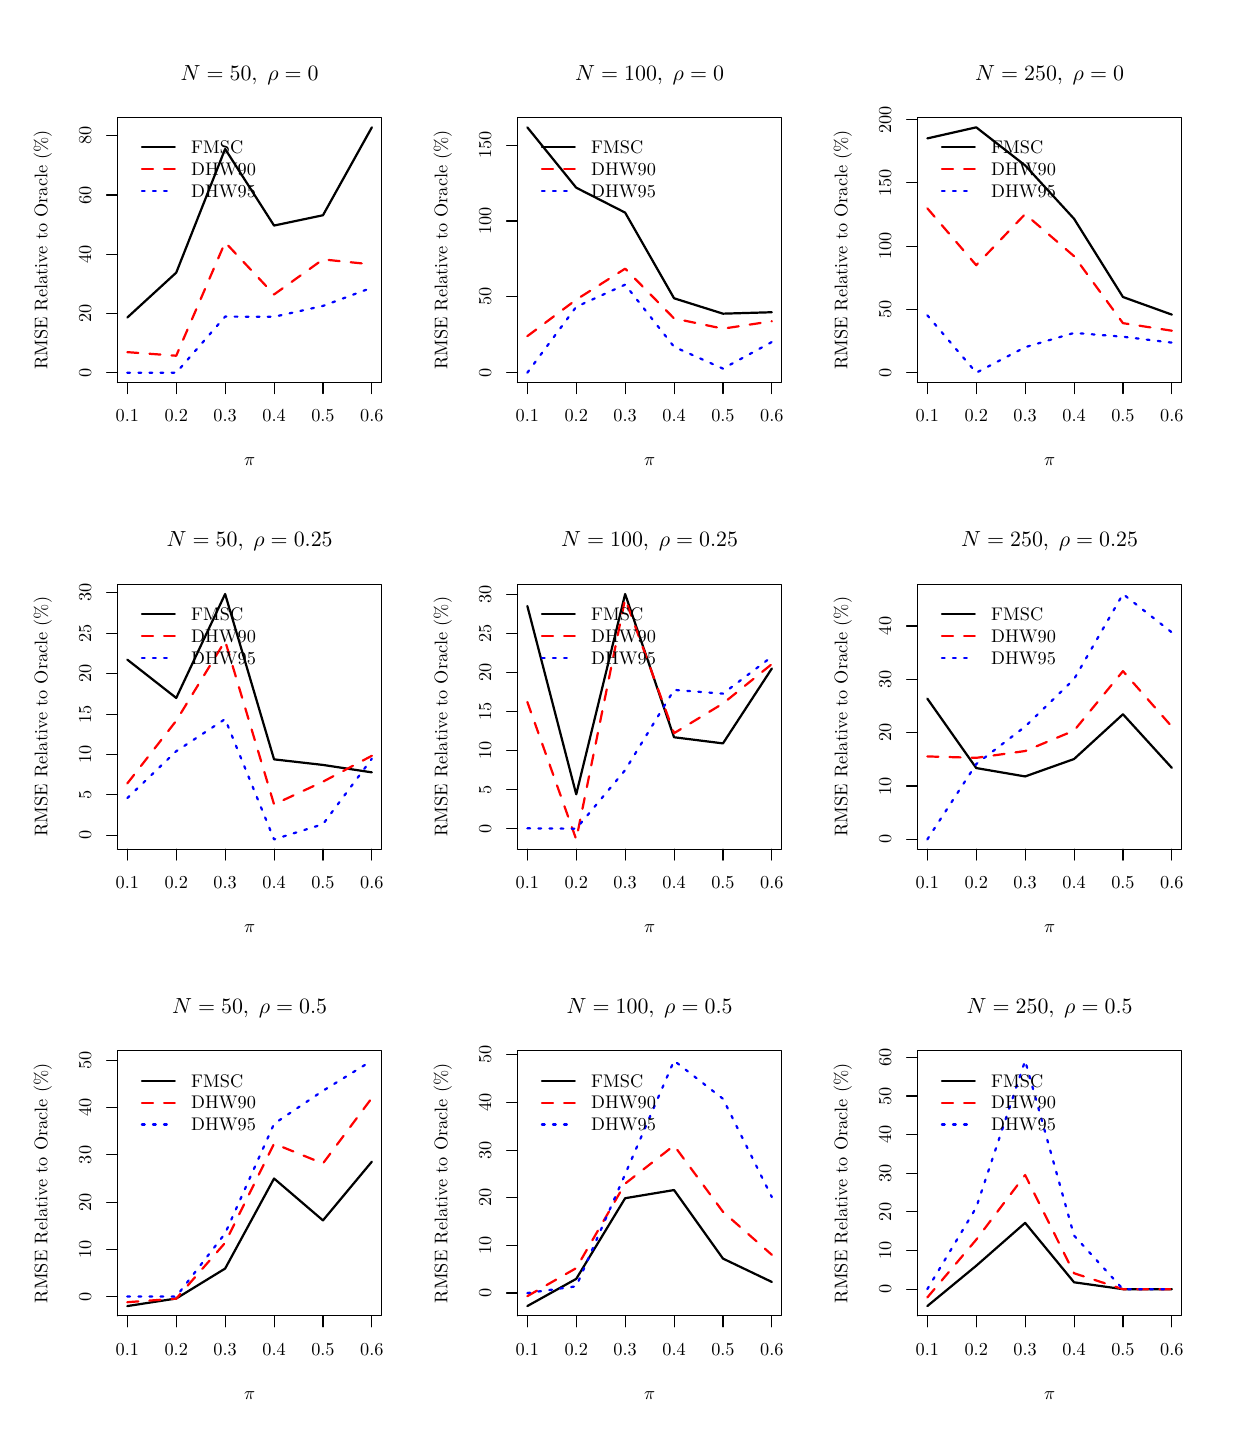
\begin{tikzpicture}[x=1pt,y=1pt]
\definecolor[named]{fillColor}{rgb}{1.00,1.00,1.00}
\path[use as bounding box,fill=fillColor,fill opacity=0.00] (0,0) rectangle (433.62,505.89);
\begin{scope}
\path[clip] ( 32.47,377.65) rectangle (127.91,473.42);
\definecolor[named]{drawColor}{rgb}{0.00,0.00,0.00}

\path[draw=drawColor,line width= 0.8pt,line join=round,line cap=round] ( 36.01,401.15) --
	( 53.68,417.36) --
	( 71.35,462.05) --
	( 89.03,434.38) --
	(106.70,438.10) --
	(124.37,469.87);
\end{scope}
\begin{scope}
\path[clip] (  0.00,  0.00) rectangle (433.62,505.89);
\definecolor[named]{drawColor}{rgb}{0.00,0.00,0.00}

\path[draw=drawColor,line width= 0.4pt,line join=round,line cap=round] ( 36.01,377.65) -- (124.37,377.65);

\path[draw=drawColor,line width= 0.4pt,line join=round,line cap=round] ( 36.01,377.65) -- ( 36.01,373.69);

\path[draw=drawColor,line width= 0.4pt,line join=round,line cap=round] ( 53.68,377.65) -- ( 53.68,373.69);

\path[draw=drawColor,line width= 0.4pt,line join=round,line cap=round] ( 71.35,377.65) -- ( 71.35,373.69);

\path[draw=drawColor,line width= 0.4pt,line join=round,line cap=round] ( 89.03,377.65) -- ( 89.03,373.69);

\path[draw=drawColor,line width= 0.4pt,line join=round,line cap=round] (106.70,377.65) -- (106.70,373.69);

\path[draw=drawColor,line width= 0.4pt,line join=round,line cap=round] (124.37,377.65) -- (124.37,373.69);

\node[text=drawColor,anchor=base,inner sep=0pt, outer sep=0pt, scale=  0.66] at ( 36.01,363.40) {0.1};

\node[text=drawColor,anchor=base,inner sep=0pt, outer sep=0pt, scale=  0.66] at ( 53.68,363.40) {0.2};

\node[text=drawColor,anchor=base,inner sep=0pt, outer sep=0pt, scale=  0.66] at ( 71.35,363.40) {0.3};

\node[text=drawColor,anchor=base,inner sep=0pt, outer sep=0pt, scale=  0.66] at ( 89.03,363.40) {0.4};

\node[text=drawColor,anchor=base,inner sep=0pt, outer sep=0pt, scale=  0.66] at (106.70,363.40) {0.5};

\node[text=drawColor,anchor=base,inner sep=0pt, outer sep=0pt, scale=  0.66] at (124.37,363.40) {0.6};

\path[draw=drawColor,line width= 0.4pt,line join=round,line cap=round] ( 32.47,381.20) -- ( 32.47,466.82);

\path[draw=drawColor,line width= 0.4pt,line join=round,line cap=round] ( 32.47,381.20) -- ( 28.51,381.20);

\path[draw=drawColor,line width= 0.4pt,line join=round,line cap=round] ( 32.47,402.61) -- ( 28.51,402.61);

\path[draw=drawColor,line width= 0.4pt,line join=round,line cap=round] ( 32.47,424.01) -- ( 28.51,424.01);

\path[draw=drawColor,line width= 0.4pt,line join=round,line cap=round] ( 32.47,445.42) -- ( 28.51,445.42);

\path[draw=drawColor,line width= 0.4pt,line join=round,line cap=round] ( 32.47,466.82) -- ( 28.51,466.82);

\node[text=drawColor,rotate= 90.00,anchor=base,inner sep=0pt, outer sep=0pt, scale=  0.66] at ( 22.97,381.20) {0};

\node[text=drawColor,rotate= 90.00,anchor=base,inner sep=0pt, outer sep=0pt, scale=  0.66] at ( 22.97,402.61) {20};

\node[text=drawColor,rotate= 90.00,anchor=base,inner sep=0pt, outer sep=0pt, scale=  0.66] at ( 22.97,424.01) {40};

\node[text=drawColor,rotate= 90.00,anchor=base,inner sep=0pt, outer sep=0pt, scale=  0.66] at ( 22.97,445.42) {60};

\node[text=drawColor,rotate= 90.00,anchor=base,inner sep=0pt, outer sep=0pt, scale=  0.66] at ( 22.97,466.82) {80};

\path[draw=drawColor,line width= 0.4pt,line join=round,line cap=round] ( 32.47,377.65) --
	(127.91,377.65) --
	(127.91,473.42) --
	( 32.47,473.42) --
	( 32.47,377.65);
\end{scope}
\begin{scope}
\path[clip] (  0.00,337.26) rectangle (144.54,505.89);
\definecolor[named]{drawColor}{rgb}{0.00,0.00,0.00}

\node[text=drawColor,anchor=base,inner sep=0pt, outer sep=0pt, scale=  0.79] at ( 80.19,486.92) {\bfseries $N=50, \;\rho=0$};

\node[text=drawColor,anchor=base,inner sep=0pt, outer sep=0pt, scale=  0.66] at ( 80.19,347.56) {$\pi$};

\node[text=drawColor,rotate= 90.00,anchor=base,inner sep=0pt, outer sep=0pt, scale=  0.66] at (  7.13,425.53) {RMSE Relative to Oracle (\%)};
\end{scope}
\begin{scope}
\path[clip] ( 32.47,377.65) rectangle (127.91,473.42);
\definecolor[named]{drawColor}{rgb}{1.00,0.00,0.00}

\path[draw=drawColor,line width= 0.8pt,dash pattern=on 4pt off 4pt ,line join=round,line cap=round] ( 36.01,388.64) --
	( 53.68,387.34) --
	( 71.35,428.32) --
	( 89.03,409.47) --
	(106.70,422.15) --
	(124.37,420.33);
\definecolor[named]{drawColor}{rgb}{0.00,0.00,1.00}

\path[draw=drawColor,line width= 0.8pt,dash pattern=on 1pt off 3pt ,line join=round,line cap=round] ( 36.01,381.20) --
	( 53.68,381.20) --
	( 71.35,401.48) --
	( 89.03,401.42) --
	(106.70,405.34) --
	(124.37,411.94);
\definecolor[named]{drawColor}{rgb}{0.00,0.00,0.00}

\path[draw=drawColor,line width= 0.8pt,line join=round,line cap=round] ( 41.28,462.63) -- ( 53.16,462.63);
\definecolor[named]{drawColor}{rgb}{1.00,0.00,0.00}

\path[draw=drawColor,line width= 0.8pt,dash pattern=on 4pt off 4pt ,line join=round,line cap=round] ( 41.28,454.71) -- ( 53.16,454.71);
\definecolor[named]{drawColor}{rgb}{0.00,0.00,1.00}

\path[draw=drawColor,line width= 0.8pt,dash pattern=on 1pt off 3pt ,line join=round,line cap=round] ( 41.28,446.79) -- ( 53.16,446.79);
\definecolor[named]{drawColor}{rgb}{0.00,0.00,0.00}

\node[text=drawColor,anchor=base west,inner sep=0pt, outer sep=0pt, scale=  0.66] at ( 59.10,460.35) {FMSC};

\node[text=drawColor,anchor=base west,inner sep=0pt, outer sep=0pt, scale=  0.66] at ( 59.10,452.43) {DHW90};

\node[text=drawColor,anchor=base west,inner sep=0pt, outer sep=0pt, scale=  0.66] at ( 59.10,444.51) {DHW95};
\end{scope}
\begin{scope}
\path[clip] (177.01,377.65) rectangle (272.45,473.42);
\definecolor[named]{drawColor}{rgb}{0.00,0.00,0.00}

\path[draw=drawColor,line width= 0.8pt,line join=round,line cap=round] (180.55,469.87) --
	(198.22,448.06) --
	(215.89,439.06) --
	(233.57,408.10) --
	(251.24,402.54) --
	(268.91,403.06);
\end{scope}
\begin{scope}
\path[clip] (  0.00,  0.00) rectangle (433.62,505.89);
\definecolor[named]{drawColor}{rgb}{0.00,0.00,0.00}

\path[draw=drawColor,line width= 0.4pt,line join=round,line cap=round] (180.55,377.65) -- (268.91,377.65);

\path[draw=drawColor,line width= 0.4pt,line join=round,line cap=round] (180.55,377.65) -- (180.55,373.69);

\path[draw=drawColor,line width= 0.4pt,line join=round,line cap=round] (198.22,377.65) -- (198.22,373.69);

\path[draw=drawColor,line width= 0.4pt,line join=round,line cap=round] (215.89,377.65) -- (215.89,373.69);

\path[draw=drawColor,line width= 0.4pt,line join=round,line cap=round] (233.57,377.65) -- (233.57,373.69);

\path[draw=drawColor,line width= 0.4pt,line join=round,line cap=round] (251.24,377.65) -- (251.24,373.69);

\path[draw=drawColor,line width= 0.4pt,line join=round,line cap=round] (268.91,377.65) -- (268.91,373.69);

\node[text=drawColor,anchor=base,inner sep=0pt, outer sep=0pt, scale=  0.66] at (180.55,363.40) {0.1};

\node[text=drawColor,anchor=base,inner sep=0pt, outer sep=0pt, scale=  0.66] at (198.22,363.40) {0.2};

\node[text=drawColor,anchor=base,inner sep=0pt, outer sep=0pt, scale=  0.66] at (215.89,363.40) {0.3};

\node[text=drawColor,anchor=base,inner sep=0pt, outer sep=0pt, scale=  0.66] at (233.57,363.40) {0.4};

\node[text=drawColor,anchor=base,inner sep=0pt, outer sep=0pt, scale=  0.66] at (251.24,363.40) {0.5};

\node[text=drawColor,anchor=base,inner sep=0pt, outer sep=0pt, scale=  0.66] at (268.91,363.40) {0.6};

\path[draw=drawColor,line width= 0.4pt,line join=round,line cap=round] (177.01,381.20) -- (177.01,463.45);

\path[draw=drawColor,line width= 0.4pt,line join=round,line cap=round] (177.01,381.20) -- (173.05,381.20);

\path[draw=drawColor,line width= 0.4pt,line join=round,line cap=round] (177.01,408.62) -- (173.05,408.62);

\path[draw=drawColor,line width= 0.4pt,line join=round,line cap=round] (177.01,436.03) -- (173.05,436.03);

\path[draw=drawColor,line width= 0.4pt,line join=round,line cap=round] (177.01,463.45) -- (173.05,463.45);

\node[text=drawColor,rotate= 90.00,anchor=base,inner sep=0pt, outer sep=0pt, scale=  0.66] at (167.51,381.20) {0};

\node[text=drawColor,rotate= 90.00,anchor=base,inner sep=0pt, outer sep=0pt, scale=  0.66] at (167.51,408.62) {50};

\node[text=drawColor,rotate= 90.00,anchor=base,inner sep=0pt, outer sep=0pt, scale=  0.66] at (167.51,436.03) {100};

\node[text=drawColor,rotate= 90.00,anchor=base,inner sep=0pt, outer sep=0pt, scale=  0.66] at (167.51,463.45) {150};

\path[draw=drawColor,line width= 0.4pt,line join=round,line cap=round] (177.01,377.65) --
	(272.45,377.65) --
	(272.45,473.42) --
	(177.01,473.42) --
	(177.01,377.65);
\end{scope}
\begin{scope}
\path[clip] (144.54,337.26) rectangle (289.08,505.89);
\definecolor[named]{drawColor}{rgb}{0.00,0.00,0.00}

\node[text=drawColor,anchor=base,inner sep=0pt, outer sep=0pt, scale=  0.79] at (224.73,486.92) {\bfseries $N=100, \;\rho=0$};

\node[text=drawColor,anchor=base,inner sep=0pt, outer sep=0pt, scale=  0.66] at (224.73,347.56) {$\pi$};

\node[text=drawColor,rotate= 90.00,anchor=base,inner sep=0pt, outer sep=0pt, scale=  0.66] at (151.67,425.53) {RMSE Relative to Oracle (\%)};
\end{scope}
\begin{scope}
\path[clip] (177.01,377.65) rectangle (272.45,473.42);
\definecolor[named]{drawColor}{rgb}{1.00,0.00,0.00}

\path[draw=drawColor,line width= 0.8pt,dash pattern=on 4pt off 4pt ,line join=round,line cap=round] (180.55,394.41) --
	(198.22,407.60) --
	(215.89,418.80) --
	(233.57,400.82) --
	(251.24,397.12) --
	(268.91,399.80);
\definecolor[named]{drawColor}{rgb}{0.00,0.00,1.00}

\path[draw=drawColor,line width= 0.8pt,dash pattern=on 1pt off 3pt ,line join=round,line cap=round] (180.55,381.20) --
	(198.22,405.02) --
	(215.89,413.03) --
	(233.57,390.56) --
	(251.24,382.69) --
	(268.91,392.30);
\definecolor[named]{drawColor}{rgb}{0.00,0.00,0.00}

\path[draw=drawColor,line width= 0.8pt,line join=round,line cap=round] (185.82,462.63) -- (197.70,462.63);
\definecolor[named]{drawColor}{rgb}{1.00,0.00,0.00}

\path[draw=drawColor,line width= 0.8pt,dash pattern=on 4pt off 4pt ,line join=round,line cap=round] (185.82,454.71) -- (197.70,454.71);
\definecolor[named]{drawColor}{rgb}{0.00,0.00,1.00}

\path[draw=drawColor,line width= 0.8pt,dash pattern=on 1pt off 3pt ,line join=round,line cap=round] (185.82,446.79) -- (197.70,446.79);
\definecolor[named]{drawColor}{rgb}{0.00,0.00,0.00}

\node[text=drawColor,anchor=base west,inner sep=0pt, outer sep=0pt, scale=  0.66] at (203.64,460.35) {FMSC};

\node[text=drawColor,anchor=base west,inner sep=0pt, outer sep=0pt, scale=  0.66] at (203.64,452.43) {DHW90};

\node[text=drawColor,anchor=base west,inner sep=0pt, outer sep=0pt, scale=  0.66] at (203.64,444.51) {DHW95};
\end{scope}
\begin{scope}
\path[clip] (321.55,377.65) rectangle (416.99,473.42);
\definecolor[named]{drawColor}{rgb}{0.00,0.00,0.00}

\path[draw=drawColor,line width= 0.8pt,line join=round,line cap=round] (325.09,465.87) --
	(342.76,469.87) --
	(360.43,456.11) --
	(378.11,436.82) --
	(395.78,408.56) --
	(413.45,402.19);
\end{scope}
\begin{scope}
\path[clip] (  0.00,  0.00) rectangle (433.62,505.89);
\definecolor[named]{drawColor}{rgb}{0.00,0.00,0.00}

\path[draw=drawColor,line width= 0.4pt,line join=round,line cap=round] (325.09,377.65) -- (413.45,377.65);

\path[draw=drawColor,line width= 0.4pt,line join=round,line cap=round] (325.09,377.65) -- (325.09,373.69);

\path[draw=drawColor,line width= 0.4pt,line join=round,line cap=round] (342.76,377.65) -- (342.76,373.69);

\path[draw=drawColor,line width= 0.4pt,line join=round,line cap=round] (360.43,377.65) -- (360.43,373.69);

\path[draw=drawColor,line width= 0.4pt,line join=round,line cap=round] (378.11,377.65) -- (378.11,373.69);

\path[draw=drawColor,line width= 0.4pt,line join=round,line cap=round] (395.78,377.65) -- (395.78,373.69);

\path[draw=drawColor,line width= 0.4pt,line join=round,line cap=round] (413.45,377.65) -- (413.45,373.69);

\node[text=drawColor,anchor=base,inner sep=0pt, outer sep=0pt, scale=  0.66] at (325.09,363.40) {0.1};

\node[text=drawColor,anchor=base,inner sep=0pt, outer sep=0pt, scale=  0.66] at (342.76,363.40) {0.2};

\node[text=drawColor,anchor=base,inner sep=0pt, outer sep=0pt, scale=  0.66] at (360.43,363.40) {0.3};

\node[text=drawColor,anchor=base,inner sep=0pt, outer sep=0pt, scale=  0.66] at (378.11,363.40) {0.4};

\node[text=drawColor,anchor=base,inner sep=0pt, outer sep=0pt, scale=  0.66] at (395.78,363.40) {0.5};

\node[text=drawColor,anchor=base,inner sep=0pt, outer sep=0pt, scale=  0.66] at (413.45,363.40) {0.6};

\path[draw=drawColor,line width= 0.4pt,line join=round,line cap=round] (321.55,381.20) -- (321.55,472.67);

\path[draw=drawColor,line width= 0.4pt,line join=round,line cap=round] (321.55,381.20) -- (317.59,381.20);

\path[draw=drawColor,line width= 0.4pt,line join=round,line cap=round] (321.55,404.07) -- (317.59,404.07);

\path[draw=drawColor,line width= 0.4pt,line join=round,line cap=round] (321.55,426.94) -- (317.59,426.94);

\path[draw=drawColor,line width= 0.4pt,line join=round,line cap=round] (321.55,449.80) -- (317.59,449.80);

\path[draw=drawColor,line width= 0.4pt,line join=round,line cap=round] (321.55,472.67) -- (317.59,472.67);

\node[text=drawColor,rotate= 90.00,anchor=base,inner sep=0pt, outer sep=0pt, scale=  0.66] at (312.05,381.20) {0};

\node[text=drawColor,rotate= 90.00,anchor=base,inner sep=0pt, outer sep=0pt, scale=  0.66] at (312.05,404.07) {50};

\node[text=drawColor,rotate= 90.00,anchor=base,inner sep=0pt, outer sep=0pt, scale=  0.66] at (312.05,426.94) {100};

\node[text=drawColor,rotate= 90.00,anchor=base,inner sep=0pt, outer sep=0pt, scale=  0.66] at (312.05,449.80) {150};

\node[text=drawColor,rotate= 90.00,anchor=base,inner sep=0pt, outer sep=0pt, scale=  0.66] at (312.05,472.67) {200};

\path[draw=drawColor,line width= 0.4pt,line join=round,line cap=round] (321.55,377.65) --
	(416.99,377.65) --
	(416.99,473.42) --
	(321.55,473.42) --
	(321.55,377.65);
\end{scope}
\begin{scope}
\path[clip] (289.08,337.26) rectangle (433.62,505.89);
\definecolor[named]{drawColor}{rgb}{0.00,0.00,0.00}

\node[text=drawColor,anchor=base,inner sep=0pt, outer sep=0pt, scale=  0.79] at (369.27,486.92) {\bfseries $N=250, \;\rho=0$};

\node[text=drawColor,anchor=base,inner sep=0pt, outer sep=0pt, scale=  0.66] at (369.27,347.56) {$\pi$};

\node[text=drawColor,rotate= 90.00,anchor=base,inner sep=0pt, outer sep=0pt, scale=  0.66] at (296.21,425.53) {RMSE Relative to Oracle (\%)};
\end{scope}
\begin{scope}
\path[clip] (321.55,377.65) rectangle (416.99,473.42);
\definecolor[named]{drawColor}{rgb}{1.00,0.00,0.00}

\path[draw=drawColor,line width= 0.8pt,dash pattern=on 4pt off 4pt ,line join=round,line cap=round] (325.09,440.61) --
	(342.76,420.05) --
	(360.43,438.52) --
	(378.11,423.30) --
	(395.78,399.11) --
	(413.45,396.38);
\definecolor[named]{drawColor}{rgb}{0.00,0.00,1.00}

\path[draw=drawColor,line width= 0.8pt,dash pattern=on 1pt off 3pt ,line join=round,line cap=round] (325.09,401.95) --
	(342.76,381.20) --
	(360.43,390.42) --
	(378.11,395.59) --
	(395.78,394.21) --
	(413.45,392.07);
\definecolor[named]{drawColor}{rgb}{0.00,0.00,0.00}

\path[draw=drawColor,line width= 0.8pt,line join=round,line cap=round] (330.36,462.63) -- (342.24,462.63);
\definecolor[named]{drawColor}{rgb}{1.00,0.00,0.00}

\path[draw=drawColor,line width= 0.8pt,dash pattern=on 4pt off 4pt ,line join=round,line cap=round] (330.36,454.71) -- (342.24,454.71);
\definecolor[named]{drawColor}{rgb}{0.00,0.00,1.00}

\path[draw=drawColor,line width= 0.8pt,dash pattern=on 1pt off 3pt ,line join=round,line cap=round] (330.36,446.79) -- (342.24,446.79);
\definecolor[named]{drawColor}{rgb}{0.00,0.00,0.00}

\node[text=drawColor,anchor=base west,inner sep=0pt, outer sep=0pt, scale=  0.66] at (348.18,460.35) {FMSC};

\node[text=drawColor,anchor=base west,inner sep=0pt, outer sep=0pt, scale=  0.66] at (348.18,452.43) {DHW90};

\node[text=drawColor,anchor=base west,inner sep=0pt, outer sep=0pt, scale=  0.66] at (348.18,444.51) {DHW95};
\end{scope}
\begin{scope}
\path[clip] ( 32.47,209.02) rectangle (127.91,304.79);
\definecolor[named]{drawColor}{rgb}{0.00,0.00,0.00}

\path[draw=drawColor,line width= 0.8pt,line join=round,line cap=round] ( 36.01,277.52) --
	( 53.68,263.68) --
	( 71.35,301.24) --
	( 89.03,241.49) --
	(106.70,239.48) --
	(124.37,236.79);
\end{scope}
\begin{scope}
\path[clip] (  0.00,  0.00) rectangle (433.62,505.89);
\definecolor[named]{drawColor}{rgb}{0.00,0.00,0.00}

\path[draw=drawColor,line width= 0.4pt,line join=round,line cap=round] ( 36.01,209.02) -- (124.37,209.02);

\path[draw=drawColor,line width= 0.4pt,line join=round,line cap=round] ( 36.01,209.02) -- ( 36.01,205.06);

\path[draw=drawColor,line width= 0.4pt,line join=round,line cap=round] ( 53.68,209.02) -- ( 53.68,205.06);

\path[draw=drawColor,line width= 0.4pt,line join=round,line cap=round] ( 71.35,209.02) -- ( 71.35,205.06);

\path[draw=drawColor,line width= 0.4pt,line join=round,line cap=round] ( 89.03,209.02) -- ( 89.03,205.06);

\path[draw=drawColor,line width= 0.4pt,line join=round,line cap=round] (106.70,209.02) -- (106.70,205.06);

\path[draw=drawColor,line width= 0.4pt,line join=round,line cap=round] (124.37,209.02) -- (124.37,205.06);

\node[text=drawColor,anchor=base,inner sep=0pt, outer sep=0pt, scale=  0.66] at ( 36.01,194.77) {0.1};

\node[text=drawColor,anchor=base,inner sep=0pt, outer sep=0pt, scale=  0.66] at ( 53.68,194.77) {0.2};

\node[text=drawColor,anchor=base,inner sep=0pt, outer sep=0pt, scale=  0.66] at ( 71.35,194.77) {0.3};

\node[text=drawColor,anchor=base,inner sep=0pt, outer sep=0pt, scale=  0.66] at ( 89.03,194.77) {0.4};

\node[text=drawColor,anchor=base,inner sep=0pt, outer sep=0pt, scale=  0.66] at (106.70,194.77) {0.5};

\node[text=drawColor,anchor=base,inner sep=0pt, outer sep=0pt, scale=  0.66] at (124.37,194.77) {0.6};

\path[draw=drawColor,line width= 0.4pt,line join=round,line cap=round] ( 32.47,214.04) -- ( 32.47,301.67);

\path[draw=drawColor,line width= 0.4pt,line join=round,line cap=round] ( 32.47,214.04) -- ( 28.51,214.04);

\path[draw=drawColor,line width= 0.4pt,line join=round,line cap=round] ( 32.47,228.65) -- ( 28.51,228.65);

\path[draw=drawColor,line width= 0.4pt,line join=round,line cap=round] ( 32.47,243.25) -- ( 28.51,243.25);

\path[draw=drawColor,line width= 0.4pt,line join=round,line cap=round] ( 32.47,257.86) -- ( 28.51,257.86);

\path[draw=drawColor,line width= 0.4pt,line join=round,line cap=round] ( 32.47,272.46) -- ( 28.51,272.46);

\path[draw=drawColor,line width= 0.4pt,line join=round,line cap=round] ( 32.47,287.07) -- ( 28.51,287.07);

\path[draw=drawColor,line width= 0.4pt,line join=round,line cap=round] ( 32.47,301.67) -- ( 28.51,301.67);

\node[text=drawColor,rotate= 90.00,anchor=base,inner sep=0pt, outer sep=0pt, scale=  0.66] at ( 22.97,214.04) {0};

\node[text=drawColor,rotate= 90.00,anchor=base,inner sep=0pt, outer sep=0pt, scale=  0.66] at ( 22.97,228.65) {5};

\node[text=drawColor,rotate= 90.00,anchor=base,inner sep=0pt, outer sep=0pt, scale=  0.66] at ( 22.97,243.25) {10};

\node[text=drawColor,rotate= 90.00,anchor=base,inner sep=0pt, outer sep=0pt, scale=  0.66] at ( 22.97,257.86) {15};

\node[text=drawColor,rotate= 90.00,anchor=base,inner sep=0pt, outer sep=0pt, scale=  0.66] at ( 22.97,272.46) {20};

\node[text=drawColor,rotate= 90.00,anchor=base,inner sep=0pt, outer sep=0pt, scale=  0.66] at ( 22.97,287.07) {25};

\node[text=drawColor,rotate= 90.00,anchor=base,inner sep=0pt, outer sep=0pt, scale=  0.66] at ( 22.97,301.67) {30};

\path[draw=drawColor,line width= 0.4pt,line join=round,line cap=round] ( 32.47,209.02) --
	(127.91,209.02) --
	(127.91,304.79) --
	( 32.47,304.79) --
	( 32.47,209.02);
\end{scope}
\begin{scope}
\path[clip] (  0.00,168.63) rectangle (144.54,337.26);
\definecolor[named]{drawColor}{rgb}{0.00,0.00,0.00}

\node[text=drawColor,anchor=base,inner sep=0pt, outer sep=0pt, scale=  0.79] at ( 80.19,318.29) {\bfseries $N=50, \;\rho=0.25$};

\node[text=drawColor,anchor=base,inner sep=0pt, outer sep=0pt, scale=  0.66] at ( 80.19,178.93) {$\pi$};

\node[text=drawColor,rotate= 90.00,anchor=base,inner sep=0pt, outer sep=0pt, scale=  0.66] at (  7.13,256.90) {RMSE Relative to Oracle (\%)};
\end{scope}
\begin{scope}
\path[clip] ( 32.47,209.02) rectangle (127.91,304.79);
\definecolor[named]{drawColor}{rgb}{1.00,0.00,0.00}

\path[draw=drawColor,line width= 0.8pt,dash pattern=on 4pt off 4pt ,line join=round,line cap=round] ( 36.01,232.79) --
	( 53.68,255.44) --
	( 71.35,284.30) --
	( 89.03,225.21) --
	(106.70,233.42) --
	(124.37,242.79);
\definecolor[named]{drawColor}{rgb}{0.00,0.00,1.00}

\path[draw=drawColor,line width= 0.8pt,dash pattern=on 1pt off 3pt ,line join=round,line cap=round] ( 36.01,227.50) --
	( 53.68,244.44) --
	( 71.35,256.05) --
	( 89.03,212.57) --
	(106.70,218.07) --
	(124.37,241.73);
\definecolor[named]{drawColor}{rgb}{0.00,0.00,0.00}

\path[draw=drawColor,line width= 0.8pt,line join=round,line cap=round] ( 41.28,294.00) -- ( 53.16,294.00);
\definecolor[named]{drawColor}{rgb}{1.00,0.00,0.00}

\path[draw=drawColor,line width= 0.8pt,dash pattern=on 4pt off 4pt ,line join=round,line cap=round] ( 41.28,286.08) -- ( 53.16,286.08);
\definecolor[named]{drawColor}{rgb}{0.00,0.00,1.00}

\path[draw=drawColor,line width= 0.8pt,dash pattern=on 1pt off 3pt ,line join=round,line cap=round] ( 41.28,278.16) -- ( 53.16,278.16);
\definecolor[named]{drawColor}{rgb}{0.00,0.00,0.00}

\node[text=drawColor,anchor=base west,inner sep=0pt, outer sep=0pt, scale=  0.66] at ( 59.10,291.72) {FMSC};

\node[text=drawColor,anchor=base west,inner sep=0pt, outer sep=0pt, scale=  0.66] at ( 59.10,283.80) {DHW90};

\node[text=drawColor,anchor=base west,inner sep=0pt, outer sep=0pt, scale=  0.66] at ( 59.10,275.88) {DHW95};
\end{scope}
\begin{scope}
\path[clip] (177.01,209.02) rectangle (272.45,304.79);
\definecolor[named]{drawColor}{rgb}{0.00,0.00,0.00}

\path[draw=drawColor,line width= 0.8pt,line join=round,line cap=round] (180.55,296.92) --
	(198.22,228.86) --
	(215.89,301.24) --
	(233.57,249.48) --
	(251.24,247.26) --
	(268.91,274.33);
\end{scope}
\begin{scope}
\path[clip] (  0.00,  0.00) rectangle (433.62,505.89);
\definecolor[named]{drawColor}{rgb}{0.00,0.00,0.00}

\path[draw=drawColor,line width= 0.4pt,line join=round,line cap=round] (180.55,209.02) -- (268.91,209.02);

\path[draw=drawColor,line width= 0.4pt,line join=round,line cap=round] (180.55,209.02) -- (180.55,205.06);

\path[draw=drawColor,line width= 0.4pt,line join=round,line cap=round] (198.22,209.02) -- (198.22,205.06);

\path[draw=drawColor,line width= 0.4pt,line join=round,line cap=round] (215.89,209.02) -- (215.89,205.06);

\path[draw=drawColor,line width= 0.4pt,line join=round,line cap=round] (233.57,209.02) -- (233.57,205.06);

\path[draw=drawColor,line width= 0.4pt,line join=round,line cap=round] (251.24,209.02) -- (251.24,205.06);

\path[draw=drawColor,line width= 0.4pt,line join=round,line cap=round] (268.91,209.02) -- (268.91,205.06);

\node[text=drawColor,anchor=base,inner sep=0pt, outer sep=0pt, scale=  0.66] at (180.55,194.77) {0.1};

\node[text=drawColor,anchor=base,inner sep=0pt, outer sep=0pt, scale=  0.66] at (198.22,194.77) {0.2};

\node[text=drawColor,anchor=base,inner sep=0pt, outer sep=0pt, scale=  0.66] at (215.89,194.77) {0.3};

\node[text=drawColor,anchor=base,inner sep=0pt, outer sep=0pt, scale=  0.66] at (233.57,194.77) {0.4};

\node[text=drawColor,anchor=base,inner sep=0pt, outer sep=0pt, scale=  0.66] at (251.24,194.77) {0.5};

\node[text=drawColor,anchor=base,inner sep=0pt, outer sep=0pt, scale=  0.66] at (268.91,194.77) {0.6};

\path[draw=drawColor,line width= 0.4pt,line join=round,line cap=round] (177.01,216.42) -- (177.01,300.97);

\path[draw=drawColor,line width= 0.4pt,line join=round,line cap=round] (177.01,216.42) -- (173.05,216.42);

\path[draw=drawColor,line width= 0.4pt,line join=round,line cap=round] (177.01,230.51) -- (173.05,230.51);

\path[draw=drawColor,line width= 0.4pt,line join=round,line cap=round] (177.01,244.61) -- (173.05,244.61);

\path[draw=drawColor,line width= 0.4pt,line join=round,line cap=round] (177.01,258.70) -- (173.05,258.70);

\path[draw=drawColor,line width= 0.4pt,line join=round,line cap=round] (177.01,272.79) -- (173.05,272.79);

\path[draw=drawColor,line width= 0.4pt,line join=round,line cap=round] (177.01,286.88) -- (173.05,286.88);

\path[draw=drawColor,line width= 0.4pt,line join=round,line cap=round] (177.01,300.97) -- (173.05,300.97);

\node[text=drawColor,rotate= 90.00,anchor=base,inner sep=0pt, outer sep=0pt, scale=  0.66] at (167.51,216.42) {0};

\node[text=drawColor,rotate= 90.00,anchor=base,inner sep=0pt, outer sep=0pt, scale=  0.66] at (167.51,230.51) {5};

\node[text=drawColor,rotate= 90.00,anchor=base,inner sep=0pt, outer sep=0pt, scale=  0.66] at (167.51,244.61) {10};

\node[text=drawColor,rotate= 90.00,anchor=base,inner sep=0pt, outer sep=0pt, scale=  0.66] at (167.51,258.70) {15};

\node[text=drawColor,rotate= 90.00,anchor=base,inner sep=0pt, outer sep=0pt, scale=  0.66] at (167.51,272.79) {20};

\node[text=drawColor,rotate= 90.00,anchor=base,inner sep=0pt, outer sep=0pt, scale=  0.66] at (167.51,286.88) {25};

\node[text=drawColor,rotate= 90.00,anchor=base,inner sep=0pt, outer sep=0pt, scale=  0.66] at (167.51,300.97) {30};

\path[draw=drawColor,line width= 0.4pt,line join=round,line cap=round] (177.01,209.02) --
	(272.45,209.02) --
	(272.45,304.79) --
	(177.01,304.79) --
	(177.01,209.02);
\end{scope}
\begin{scope}
\path[clip] (144.54,168.63) rectangle (289.08,337.26);
\definecolor[named]{drawColor}{rgb}{0.00,0.00,0.00}

\node[text=drawColor,anchor=base,inner sep=0pt, outer sep=0pt, scale=  0.79] at (224.73,318.29) {\bfseries $N=100, \;\rho=0.25$};

\node[text=drawColor,anchor=base,inner sep=0pt, outer sep=0pt, scale=  0.66] at (224.73,178.93) {$\pi$};

\node[text=drawColor,rotate= 90.00,anchor=base,inner sep=0pt, outer sep=0pt, scale=  0.66] at (151.67,256.90) {RMSE Relative to Oracle (\%)};
\end{scope}
\begin{scope}
\path[clip] (177.01,209.02) rectangle (272.45,304.79);
\definecolor[named]{drawColor}{rgb}{1.00,0.00,0.00}

\path[draw=drawColor,line width= 0.8pt,dash pattern=on 4pt off 4pt ,line join=round,line cap=round] (180.55,262.23) --
	(198.22,212.57) --
	(215.89,299.52) --
	(233.57,250.94) --
	(251.24,261.67) --
	(268.91,275.93);
\definecolor[named]{drawColor}{rgb}{0.00,0.00,1.00}

\path[draw=drawColor,line width= 0.8pt,dash pattern=on 1pt off 3pt ,line join=round,line cap=round] (180.55,216.57) --
	(198.22,216.43) --
	(215.89,237.59) --
	(233.57,266.59) --
	(251.24,265.24) --
	(268.91,278.60);
\definecolor[named]{drawColor}{rgb}{0.00,0.00,0.00}

\path[draw=drawColor,line width= 0.8pt,line join=round,line cap=round] (185.82,294.00) -- (197.70,294.00);
\definecolor[named]{drawColor}{rgb}{1.00,0.00,0.00}

\path[draw=drawColor,line width= 0.8pt,dash pattern=on 4pt off 4pt ,line join=round,line cap=round] (185.82,286.08) -- (197.70,286.08);
\definecolor[named]{drawColor}{rgb}{0.00,0.00,1.00}

\path[draw=drawColor,line width= 0.8pt,dash pattern=on 1pt off 3pt ,line join=round,line cap=round] (185.82,278.16) -- (197.70,278.16);
\definecolor[named]{drawColor}{rgb}{0.00,0.00,0.00}

\node[text=drawColor,anchor=base west,inner sep=0pt, outer sep=0pt, scale=  0.66] at (203.64,291.72) {FMSC};

\node[text=drawColor,anchor=base west,inner sep=0pt, outer sep=0pt, scale=  0.66] at (203.64,283.80) {DHW90};

\node[text=drawColor,anchor=base west,inner sep=0pt, outer sep=0pt, scale=  0.66] at (203.64,275.88) {DHW95};
\end{scope}
\begin{scope}
\path[clip] (321.55,209.02) rectangle (416.99,304.79);
\definecolor[named]{drawColor}{rgb}{0.00,0.00,0.00}

\path[draw=drawColor,line width= 0.8pt,line join=round,line cap=round] (325.09,263.44) --
	(342.76,238.35) --
	(360.43,235.32) --
	(378.11,241.61) --
	(395.78,257.79) --
	(413.45,238.40);
\end{scope}
\begin{scope}
\path[clip] (  0.00,  0.00) rectangle (433.62,505.89);
\definecolor[named]{drawColor}{rgb}{0.00,0.00,0.00}

\path[draw=drawColor,line width= 0.4pt,line join=round,line cap=round] (325.09,209.02) -- (413.45,209.02);

\path[draw=drawColor,line width= 0.4pt,line join=round,line cap=round] (325.09,209.02) -- (325.09,205.06);

\path[draw=drawColor,line width= 0.4pt,line join=round,line cap=round] (342.76,209.02) -- (342.76,205.06);

\path[draw=drawColor,line width= 0.4pt,line join=round,line cap=round] (360.43,209.02) -- (360.43,205.06);

\path[draw=drawColor,line width= 0.4pt,line join=round,line cap=round] (378.11,209.02) -- (378.11,205.06);

\path[draw=drawColor,line width= 0.4pt,line join=round,line cap=round] (395.78,209.02) -- (395.78,205.06);

\path[draw=drawColor,line width= 0.4pt,line join=round,line cap=round] (413.45,209.02) -- (413.45,205.06);

\node[text=drawColor,anchor=base,inner sep=0pt, outer sep=0pt, scale=  0.66] at (325.09,194.77) {0.1};

\node[text=drawColor,anchor=base,inner sep=0pt, outer sep=0pt, scale=  0.66] at (342.76,194.77) {0.2};

\node[text=drawColor,anchor=base,inner sep=0pt, outer sep=0pt, scale=  0.66] at (360.43,194.77) {0.3};

\node[text=drawColor,anchor=base,inner sep=0pt, outer sep=0pt, scale=  0.66] at (378.11,194.77) {0.4};

\node[text=drawColor,anchor=base,inner sep=0pt, outer sep=0pt, scale=  0.66] at (395.78,194.77) {0.5};

\node[text=drawColor,anchor=base,inner sep=0pt, outer sep=0pt, scale=  0.66] at (413.45,194.77) {0.6};

\path[draw=drawColor,line width= 0.4pt,line join=round,line cap=round] (321.55,212.57) -- (321.55,289.69);

\path[draw=drawColor,line width= 0.4pt,line join=round,line cap=round] (321.55,212.57) -- (317.59,212.57);

\path[draw=drawColor,line width= 0.4pt,line join=round,line cap=round] (321.55,231.85) -- (317.59,231.85);

\path[draw=drawColor,line width= 0.4pt,line join=round,line cap=round] (321.55,251.13) -- (317.59,251.13);

\path[draw=drawColor,line width= 0.4pt,line join=round,line cap=round] (321.55,270.41) -- (317.59,270.41);

\path[draw=drawColor,line width= 0.4pt,line join=round,line cap=round] (321.55,289.69) -- (317.59,289.69);

\node[text=drawColor,rotate= 90.00,anchor=base,inner sep=0pt, outer sep=0pt, scale=  0.66] at (312.05,212.57) {0};

\node[text=drawColor,rotate= 90.00,anchor=base,inner sep=0pt, outer sep=0pt, scale=  0.66] at (312.05,231.85) {10};

\node[text=drawColor,rotate= 90.00,anchor=base,inner sep=0pt, outer sep=0pt, scale=  0.66] at (312.05,251.13) {20};

\node[text=drawColor,rotate= 90.00,anchor=base,inner sep=0pt, outer sep=0pt, scale=  0.66] at (312.05,270.41) {30};

\node[text=drawColor,rotate= 90.00,anchor=base,inner sep=0pt, outer sep=0pt, scale=  0.66] at (312.05,289.69) {40};

\path[draw=drawColor,line width= 0.4pt,line join=round,line cap=round] (321.55,209.02) --
	(416.99,209.02) --
	(416.99,304.79) --
	(321.55,304.79) --
	(321.55,209.02);
\end{scope}
\begin{scope}
\path[clip] (289.08,168.63) rectangle (433.62,337.26);
\definecolor[named]{drawColor}{rgb}{0.00,0.00,0.00}

\node[text=drawColor,anchor=base,inner sep=0pt, outer sep=0pt, scale=  0.79] at (369.27,318.29) {\bfseries $N=250, \;\rho=0.25$};

\node[text=drawColor,anchor=base,inner sep=0pt, outer sep=0pt, scale=  0.66] at (369.27,178.93) {$\pi$};

\node[text=drawColor,rotate= 90.00,anchor=base,inner sep=0pt, outer sep=0pt, scale=  0.66] at (296.21,256.90) {RMSE Relative to Oracle (\%)};
\end{scope}
\begin{scope}
\path[clip] (321.55,209.02) rectangle (416.99,304.79);
\definecolor[named]{drawColor}{rgb}{1.00,0.00,0.00}

\path[draw=drawColor,line width= 0.8pt,dash pattern=on 4pt off 4pt ,line join=round,line cap=round] (325.09,242.55) --
	(342.76,242.04) --
	(360.43,244.50) --
	(378.11,251.88) --
	(395.78,273.37) --
	(413.45,253.30);
\definecolor[named]{drawColor}{rgb}{0.00,0.00,1.00}

\path[draw=drawColor,line width= 0.8pt,dash pattern=on 1pt off 3pt ,line join=round,line cap=round] (325.09,212.57) --
	(342.76,239.80) --
	(360.43,253.34) --
	(378.11,270.47) --
	(395.78,301.24) --
	(413.45,287.35);
\definecolor[named]{drawColor}{rgb}{0.00,0.00,0.00}

\path[draw=drawColor,line width= 0.8pt,line join=round,line cap=round] (330.36,294.00) -- (342.24,294.00);
\definecolor[named]{drawColor}{rgb}{1.00,0.00,0.00}

\path[draw=drawColor,line width= 0.8pt,dash pattern=on 4pt off 4pt ,line join=round,line cap=round] (330.36,286.08) -- (342.24,286.08);
\definecolor[named]{drawColor}{rgb}{0.00,0.00,1.00}

\path[draw=drawColor,line width= 0.8pt,dash pattern=on 1pt off 3pt ,line join=round,line cap=round] (330.36,278.16) -- (342.24,278.16);
\definecolor[named]{drawColor}{rgb}{0.00,0.00,0.00}

\node[text=drawColor,anchor=base west,inner sep=0pt, outer sep=0pt, scale=  0.66] at (348.18,291.72) {FMSC};

\node[text=drawColor,anchor=base west,inner sep=0pt, outer sep=0pt, scale=  0.66] at (348.18,283.80) {DHW90};

\node[text=drawColor,anchor=base west,inner sep=0pt, outer sep=0pt, scale=  0.66] at (348.18,275.88) {DHW95};
\end{scope}
\begin{scope}
\path[clip] ( 32.47, 40.39) rectangle (127.91,136.16);
\definecolor[named]{drawColor}{rgb}{0.00,0.00,0.00}

\path[draw=drawColor,line width= 0.8pt,line join=round,line cap=round] ( 36.01, 43.94) --
	( 53.68, 46.67) --
	( 71.35, 57.49) --
	( 89.03, 90.03) --
	(106.70, 74.90) --
	(124.37, 96.12);
\end{scope}
\begin{scope}
\path[clip] (  0.00,  0.00) rectangle (433.62,505.89);
\definecolor[named]{drawColor}{rgb}{0.00,0.00,0.00}

\path[draw=drawColor,line width= 0.4pt,line join=round,line cap=round] ( 36.01, 40.39) -- (124.37, 40.39);

\path[draw=drawColor,line width= 0.4pt,line join=round,line cap=round] ( 36.01, 40.39) -- ( 36.01, 36.43);

\path[draw=drawColor,line width= 0.4pt,line join=round,line cap=round] ( 53.68, 40.39) -- ( 53.68, 36.43);

\path[draw=drawColor,line width= 0.4pt,line join=round,line cap=round] ( 71.35, 40.39) -- ( 71.35, 36.43);

\path[draw=drawColor,line width= 0.4pt,line join=round,line cap=round] ( 89.03, 40.39) -- ( 89.03, 36.43);

\path[draw=drawColor,line width= 0.4pt,line join=round,line cap=round] (106.70, 40.39) -- (106.70, 36.43);

\path[draw=drawColor,line width= 0.4pt,line join=round,line cap=round] (124.37, 40.39) -- (124.37, 36.43);

\node[text=drawColor,anchor=base,inner sep=0pt, outer sep=0pt, scale=  0.66] at ( 36.01, 26.14) {0.1};

\node[text=drawColor,anchor=base,inner sep=0pt, outer sep=0pt, scale=  0.66] at ( 53.68, 26.14) {0.2};

\node[text=drawColor,anchor=base,inner sep=0pt, outer sep=0pt, scale=  0.66] at ( 71.35, 26.14) {0.3};

\node[text=drawColor,anchor=base,inner sep=0pt, outer sep=0pt, scale=  0.66] at ( 89.03, 26.14) {0.4};

\node[text=drawColor,anchor=base,inner sep=0pt, outer sep=0pt, scale=  0.66] at (106.70, 26.14) {0.5};

\node[text=drawColor,anchor=base,inner sep=0pt, outer sep=0pt, scale=  0.66] at (124.37, 26.14) {0.6};

\path[draw=drawColor,line width= 0.4pt,line join=round,line cap=round] ( 32.47, 47.39) -- ( 32.47,132.66);

\path[draw=drawColor,line width= 0.4pt,line join=round,line cap=round] ( 32.47, 47.39) -- ( 28.51, 47.39);

\path[draw=drawColor,line width= 0.4pt,line join=round,line cap=round] ( 32.47, 64.45) -- ( 28.51, 64.45);

\path[draw=drawColor,line width= 0.4pt,line join=round,line cap=round] ( 32.47, 81.50) -- ( 28.51, 81.50);

\path[draw=drawColor,line width= 0.4pt,line join=round,line cap=round] ( 32.47, 98.55) -- ( 28.51, 98.55);

\path[draw=drawColor,line width= 0.4pt,line join=round,line cap=round] ( 32.47,115.60) -- ( 28.51,115.60);

\path[draw=drawColor,line width= 0.4pt,line join=round,line cap=round] ( 32.47,132.66) -- ( 28.51,132.66);

\node[text=drawColor,rotate= 90.00,anchor=base,inner sep=0pt, outer sep=0pt, scale=  0.66] at ( 22.97, 47.39) {0};

\node[text=drawColor,rotate= 90.00,anchor=base,inner sep=0pt, outer sep=0pt, scale=  0.66] at ( 22.97, 64.45) {10};

\node[text=drawColor,rotate= 90.00,anchor=base,inner sep=0pt, outer sep=0pt, scale=  0.66] at ( 22.97, 81.50) {20};

\node[text=drawColor,rotate= 90.00,anchor=base,inner sep=0pt, outer sep=0pt, scale=  0.66] at ( 22.97, 98.55) {30};

\node[text=drawColor,rotate= 90.00,anchor=base,inner sep=0pt, outer sep=0pt, scale=  0.66] at ( 22.97,115.60) {40};

\node[text=drawColor,rotate= 90.00,anchor=base,inner sep=0pt, outer sep=0pt, scale=  0.66] at ( 22.97,132.66) {50};

\path[draw=drawColor,line width= 0.4pt,line join=round,line cap=round] ( 32.47, 40.39) --
	(127.91, 40.39) --
	(127.91,136.16) --
	( 32.47,136.16) --
	( 32.47, 40.39);
\end{scope}
\begin{scope}
\path[clip] (  0.00,  0.00) rectangle (144.54,168.63);
\definecolor[named]{drawColor}{rgb}{0.00,0.00,0.00}

\node[text=drawColor,anchor=base,inner sep=0pt, outer sep=0pt, scale=  0.79] at ( 80.19,149.66) {\bfseries $N=50, \;\rho=0.5$};

\node[text=drawColor,anchor=base,inner sep=0pt, outer sep=0pt, scale=  0.66] at ( 80.19, 10.30) {$\pi$};

\node[text=drawColor,rotate= 90.00,anchor=base,inner sep=0pt, outer sep=0pt, scale=  0.66] at (  7.13, 88.27) {RMSE Relative to Oracle (\%)};
\end{scope}
\begin{scope}
\path[clip] ( 32.47, 40.39) rectangle (127.91,136.16);
\definecolor[named]{drawColor}{rgb}{1.00,0.00,0.00}

\path[draw=drawColor,line width= 0.8pt,dash pattern=on 4pt off 4pt ,line join=round,line cap=round] ( 36.01, 45.34) --
	( 53.68, 46.62) --
	( 71.35, 66.80) --
	( 89.03,102.63) --
	(106.70, 95.47) --
	(124.37,119.14);
\definecolor[named]{drawColor}{rgb}{0.00,0.00,1.00}

\path[draw=drawColor,line width= 0.8pt,dash pattern=on 1pt off 3pt ,line join=round,line cap=round] ( 36.01, 47.39) --
	( 53.68, 47.39) --
	( 71.35, 70.21) --
	( 89.03,109.79) --
	(106.70,121.73) --
	(124.37,132.61);
\definecolor[named]{drawColor}{rgb}{0.00,0.00,0.00}

\path[draw=drawColor,line width= 0.8pt,line join=round,line cap=round] ( 41.28,125.37) -- ( 53.16,125.37);
\definecolor[named]{drawColor}{rgb}{1.00,0.00,0.00}

\path[draw=drawColor,line width= 0.8pt,dash pattern=on 4pt off 4pt ,line join=round,line cap=round] ( 41.28,117.45) -- ( 53.16,117.45);
\definecolor[named]{drawColor}{rgb}{0.00,0.00,1.00}

\path[draw=drawColor,line width= 0.8pt,dash pattern=on 1pt off 3pt ,line join=round,line cap=round] ( 41.28,109.53) -- ( 53.16,109.53);
\definecolor[named]{drawColor}{rgb}{0.00,0.00,0.00}

\node[text=drawColor,anchor=base west,inner sep=0pt, outer sep=0pt, scale=  0.66] at ( 59.10,123.09) {FMSC};

\node[text=drawColor,anchor=base west,inner sep=0pt, outer sep=0pt, scale=  0.66] at ( 59.10,115.17) {DHW90};

\node[text=drawColor,anchor=base west,inner sep=0pt, outer sep=0pt, scale=  0.66] at ( 59.10,107.25) {DHW95};
\end{scope}
\begin{scope}
\path[clip] (177.01, 40.39) rectangle (272.45,136.16);
\definecolor[named]{drawColor}{rgb}{0.00,0.00,0.00}

\path[draw=drawColor,line width= 0.8pt,line join=round,line cap=round] (180.55, 43.94) --
	(198.22, 53.77) --
	(215.89, 82.91) --
	(233.57, 85.86) --
	(251.24, 61.10) --
	(268.91, 52.65);
\end{scope}
\begin{scope}
\path[clip] (  0.00,  0.00) rectangle (433.62,505.89);
\definecolor[named]{drawColor}{rgb}{0.00,0.00,0.00}

\path[draw=drawColor,line width= 0.4pt,line join=round,line cap=round] (180.55, 40.39) -- (268.91, 40.39);

\path[draw=drawColor,line width= 0.4pt,line join=round,line cap=round] (180.55, 40.39) -- (180.55, 36.43);

\path[draw=drawColor,line width= 0.4pt,line join=round,line cap=round] (198.22, 40.39) -- (198.22, 36.43);

\path[draw=drawColor,line width= 0.4pt,line join=round,line cap=round] (215.89, 40.39) -- (215.89, 36.43);

\path[draw=drawColor,line width= 0.4pt,line join=round,line cap=round] (233.57, 40.39) -- (233.57, 36.43);

\path[draw=drawColor,line width= 0.4pt,line join=round,line cap=round] (251.24, 40.39) -- (251.24, 36.43);

\path[draw=drawColor,line width= 0.4pt,line join=round,line cap=round] (268.91, 40.39) -- (268.91, 36.43);

\node[text=drawColor,anchor=base,inner sep=0pt, outer sep=0pt, scale=  0.66] at (180.55, 26.14) {0.1};

\node[text=drawColor,anchor=base,inner sep=0pt, outer sep=0pt, scale=  0.66] at (198.22, 26.14) {0.2};

\node[text=drawColor,anchor=base,inner sep=0pt, outer sep=0pt, scale=  0.66] at (215.89, 26.14) {0.3};

\node[text=drawColor,anchor=base,inner sep=0pt, outer sep=0pt, scale=  0.66] at (233.57, 26.14) {0.4};

\node[text=drawColor,anchor=base,inner sep=0pt, outer sep=0pt, scale=  0.66] at (251.24, 26.14) {0.5};

\node[text=drawColor,anchor=base,inner sep=0pt, outer sep=0pt, scale=  0.66] at (268.91, 26.14) {0.6};

\path[draw=drawColor,line width= 0.4pt,line join=round,line cap=round] (177.01, 48.65) -- (177.01,134.74);

\path[draw=drawColor,line width= 0.4pt,line join=round,line cap=round] (177.01, 48.65) -- (173.05, 48.65);

\path[draw=drawColor,line width= 0.4pt,line join=round,line cap=round] (177.01, 65.87) -- (173.05, 65.87);

\path[draw=drawColor,line width= 0.4pt,line join=round,line cap=round] (177.01, 83.09) -- (173.05, 83.09);

\path[draw=drawColor,line width= 0.4pt,line join=round,line cap=round] (177.01,100.30) -- (173.05,100.30);

\path[draw=drawColor,line width= 0.4pt,line join=round,line cap=round] (177.01,117.52) -- (173.05,117.52);

\path[draw=drawColor,line width= 0.4pt,line join=round,line cap=round] (177.01,134.74) -- (173.05,134.74);

\node[text=drawColor,rotate= 90.00,anchor=base,inner sep=0pt, outer sep=0pt, scale=  0.66] at (167.51, 48.65) {0};

\node[text=drawColor,rotate= 90.00,anchor=base,inner sep=0pt, outer sep=0pt, scale=  0.66] at (167.51, 65.87) {10};

\node[text=drawColor,rotate= 90.00,anchor=base,inner sep=0pt, outer sep=0pt, scale=  0.66] at (167.51, 83.09) {20};

\node[text=drawColor,rotate= 90.00,anchor=base,inner sep=0pt, outer sep=0pt, scale=  0.66] at (167.51,100.30) {30};

\node[text=drawColor,rotate= 90.00,anchor=base,inner sep=0pt, outer sep=0pt, scale=  0.66] at (167.51,117.52) {40};

\node[text=drawColor,rotate= 90.00,anchor=base,inner sep=0pt, outer sep=0pt, scale=  0.66] at (167.51,134.74) {50};

\path[draw=drawColor,line width= 0.4pt,line join=round,line cap=round] (177.01, 40.39) --
	(272.45, 40.39) --
	(272.45,136.16) --
	(177.01,136.16) --
	(177.01, 40.39);
\end{scope}
\begin{scope}
\path[clip] (144.54,  0.00) rectangle (289.08,168.63);
\definecolor[named]{drawColor}{rgb}{0.00,0.00,0.00}

\node[text=drawColor,anchor=base,inner sep=0pt, outer sep=0pt, scale=  0.79] at (224.73,149.66) {\bfseries $N=100, \;\rho=0.5$};

\node[text=drawColor,anchor=base,inner sep=0pt, outer sep=0pt, scale=  0.66] at (224.73, 10.30) {$\pi$};

\node[text=drawColor,rotate= 90.00,anchor=base,inner sep=0pt, outer sep=0pt, scale=  0.66] at (151.67, 88.27) {RMSE Relative to Oracle (\%)};
\end{scope}
\begin{scope}
\path[clip] (177.01, 40.39) rectangle (272.45,136.16);
\definecolor[named]{drawColor}{rgb}{1.00,0.00,0.00}

\path[draw=drawColor,line width= 0.8pt,dash pattern=on 4pt off 4pt ,line join=round,line cap=round] (180.55, 47.52) --
	(198.22, 57.66) --
	(215.89, 88.18) --
	(233.57,101.96) --
	(251.24, 78.01) --
	(268.91, 62.45);
\definecolor[named]{drawColor}{rgb}{0.00,0.00,1.00}

\path[draw=drawColor,line width= 0.8pt,dash pattern=on 1pt off 3pt ,line join=round,line cap=round] (180.55, 48.65) --
	(198.22, 51.08) --
	(215.89, 91.58) --
	(233.57,132.61) --
	(251.24,118.84) --
	(268.91, 83.29);
\definecolor[named]{drawColor}{rgb}{0.00,0.00,0.00}

\path[draw=drawColor,line width= 0.8pt,line join=round,line cap=round] (185.82,125.37) -- (197.70,125.37);
\definecolor[named]{drawColor}{rgb}{1.00,0.00,0.00}

\path[draw=drawColor,line width= 0.8pt,dash pattern=on 4pt off 4pt ,line join=round,line cap=round] (185.82,117.45) -- (197.70,117.45);
\definecolor[named]{drawColor}{rgb}{0.00,0.00,1.00}

\path[draw=drawColor,line width= 0.8pt,dash pattern=on 1pt off 3pt ,line join=round,line cap=round] (185.82,109.53) -- (197.70,109.53);
\definecolor[named]{drawColor}{rgb}{0.00,0.00,0.00}

\node[text=drawColor,anchor=base west,inner sep=0pt, outer sep=0pt, scale=  0.66] at (203.64,123.09) {FMSC};

\node[text=drawColor,anchor=base west,inner sep=0pt, outer sep=0pt, scale=  0.66] at (203.64,115.17) {DHW90};

\node[text=drawColor,anchor=base west,inner sep=0pt, outer sep=0pt, scale=  0.66] at (203.64,107.25) {DHW95};
\end{scope}
\begin{scope}
\path[clip] (321.55, 40.39) rectangle (416.99,136.16);
\definecolor[named]{drawColor}{rgb}{0.00,0.00,0.00}

\path[draw=drawColor,line width= 0.8pt,line join=round,line cap=round] (325.09, 43.94) --
	(342.76, 58.51) --
	(360.43, 74.00) --
	(378.11, 52.53) --
	(395.78, 50.05) --
	(413.45, 50.05);
\end{scope}
\begin{scope}
\path[clip] (  0.00,  0.00) rectangle (433.62,505.89);
\definecolor[named]{drawColor}{rgb}{0.00,0.00,0.00}

\path[draw=drawColor,line width= 0.4pt,line join=round,line cap=round] (325.09, 40.39) -- (413.45, 40.39);

\path[draw=drawColor,line width= 0.4pt,line join=round,line cap=round] (325.09, 40.39) -- (325.09, 36.43);

\path[draw=drawColor,line width= 0.4pt,line join=round,line cap=round] (342.76, 40.39) -- (342.76, 36.43);

\path[draw=drawColor,line width= 0.4pt,line join=round,line cap=round] (360.43, 40.39) -- (360.43, 36.43);

\path[draw=drawColor,line width= 0.4pt,line join=round,line cap=round] (378.11, 40.39) -- (378.11, 36.43);

\path[draw=drawColor,line width= 0.4pt,line join=round,line cap=round] (395.78, 40.39) -- (395.78, 36.43);

\path[draw=drawColor,line width= 0.4pt,line join=round,line cap=round] (413.45, 40.39) -- (413.45, 36.43);

\node[text=drawColor,anchor=base,inner sep=0pt, outer sep=0pt, scale=  0.66] at (325.09, 26.14) {0.1};

\node[text=drawColor,anchor=base,inner sep=0pt, outer sep=0pt, scale=  0.66] at (342.76, 26.14) {0.2};

\node[text=drawColor,anchor=base,inner sep=0pt, outer sep=0pt, scale=  0.66] at (360.43, 26.14) {0.3};

\node[text=drawColor,anchor=base,inner sep=0pt, outer sep=0pt, scale=  0.66] at (378.11, 26.14) {0.4};

\node[text=drawColor,anchor=base,inner sep=0pt, outer sep=0pt, scale=  0.66] at (395.78, 26.14) {0.5};

\node[text=drawColor,anchor=base,inner sep=0pt, outer sep=0pt, scale=  0.66] at (413.45, 26.14) {0.6};

\path[draw=drawColor,line width= 0.4pt,line join=round,line cap=round] (321.55, 50.05) -- (321.55,133.79);

\path[draw=drawColor,line width= 0.4pt,line join=round,line cap=round] (321.55, 50.05) -- (317.59, 50.05);

\path[draw=drawColor,line width= 0.4pt,line join=round,line cap=round] (321.55, 64.01) -- (317.59, 64.01);

\path[draw=drawColor,line width= 0.4pt,line join=round,line cap=round] (321.55, 77.97) -- (317.59, 77.97);

\path[draw=drawColor,line width= 0.4pt,line join=round,line cap=round] (321.55, 91.92) -- (317.59, 91.92);

\path[draw=drawColor,line width= 0.4pt,line join=round,line cap=round] (321.55,105.88) -- (317.59,105.88);

\path[draw=drawColor,line width= 0.4pt,line join=round,line cap=round] (321.55,119.84) -- (317.59,119.84);

\path[draw=drawColor,line width= 0.4pt,line join=round,line cap=round] (321.55,133.79) -- (317.59,133.79);

\node[text=drawColor,rotate= 90.00,anchor=base,inner sep=0pt, outer sep=0pt, scale=  0.66] at (312.05, 50.05) {0};

\node[text=drawColor,rotate= 90.00,anchor=base,inner sep=0pt, outer sep=0pt, scale=  0.66] at (312.05, 64.01) {10};

\node[text=drawColor,rotate= 90.00,anchor=base,inner sep=0pt, outer sep=0pt, scale=  0.66] at (312.05, 77.97) {20};

\node[text=drawColor,rotate= 90.00,anchor=base,inner sep=0pt, outer sep=0pt, scale=  0.66] at (312.05, 91.92) {30};

\node[text=drawColor,rotate= 90.00,anchor=base,inner sep=0pt, outer sep=0pt, scale=  0.66] at (312.05,105.88) {40};

\node[text=drawColor,rotate= 90.00,anchor=base,inner sep=0pt, outer sep=0pt, scale=  0.66] at (312.05,119.84) {50};

\node[text=drawColor,rotate= 90.00,anchor=base,inner sep=0pt, outer sep=0pt, scale=  0.66] at (312.05,133.79) {60};

\path[draw=drawColor,line width= 0.4pt,line join=round,line cap=round] (321.55, 40.39) --
	(416.99, 40.39) --
	(416.99,136.16) --
	(321.55,136.16) --
	(321.55, 40.39);
\end{scope}
\begin{scope}
\path[clip] (289.08,  0.00) rectangle (433.62,168.63);
\definecolor[named]{drawColor}{rgb}{0.00,0.00,0.00}

\node[text=drawColor,anchor=base,inner sep=0pt, outer sep=0pt, scale=  0.79] at (369.27,149.66) {\bfseries $N=250, \;\rho=0.5$};

\node[text=drawColor,anchor=base,inner sep=0pt, outer sep=0pt, scale=  0.66] at (369.27, 10.30) {$\pi$};

\node[text=drawColor,rotate= 90.00,anchor=base,inner sep=0pt, outer sep=0pt, scale=  0.66] at (296.21, 88.27) {RMSE Relative to Oracle (\%)};
\end{scope}
\begin{scope}
\path[clip] (321.55, 40.39) rectangle (416.99,136.16);
\definecolor[named]{drawColor}{rgb}{1.00,0.00,0.00}

\path[draw=drawColor,line width= 0.8pt,dash pattern=on 4pt off 4pt ,line join=round,line cap=round] (325.09, 47.05) --
	(342.76, 67.93) --
	(360.43, 91.29) --
	(378.11, 55.80) --
	(395.78, 50.05) --
	(413.45, 50.05);
\definecolor[named]{drawColor}{rgb}{0.00,0.00,1.00}

\path[draw=drawColor,line width= 0.8pt,dash pattern=on 1pt off 3pt ,line join=round,line cap=round] (325.09, 50.05) --
	(342.76, 79.55) --
	(360.43,132.61) --
	(378.11, 69.41) --
	(395.78, 50.05) --
	(413.45, 50.05);
\definecolor[named]{drawColor}{rgb}{0.00,0.00,0.00}

\path[draw=drawColor,line width= 0.8pt,line join=round,line cap=round] (330.36,125.37) -- (342.24,125.37);
\definecolor[named]{drawColor}{rgb}{1.00,0.00,0.00}

\path[draw=drawColor,line width= 0.8pt,dash pattern=on 4pt off 4pt ,line join=round,line cap=round] (330.36,117.45) -- (342.24,117.45);
\definecolor[named]{drawColor}{rgb}{0.00,0.00,1.00}

\path[draw=drawColor,line width= 0.8pt,dash pattern=on 1pt off 3pt ,line join=round,line cap=round] (330.36,109.53) -- (342.24,109.53);
\definecolor[named]{drawColor}{rgb}{0.00,0.00,0.00}

\node[text=drawColor,anchor=base west,inner sep=0pt, outer sep=0pt, scale=  0.66] at (348.18,123.09) {FMSC};

\node[text=drawColor,anchor=base west,inner sep=0pt, outer sep=0pt, scale=  0.66] at (348.18,115.17) {DHW90};

\node[text=drawColor,anchor=base west,inner sep=0pt, outer sep=0pt, scale=  0.66] at (348.18,107.25) {DHW95};
\end{scope}
\end{tikzpicture}
